\documentclass[tikz]{standalone}

\usetikzlibrary{arrows.meta,patterns}

\begin{document}
	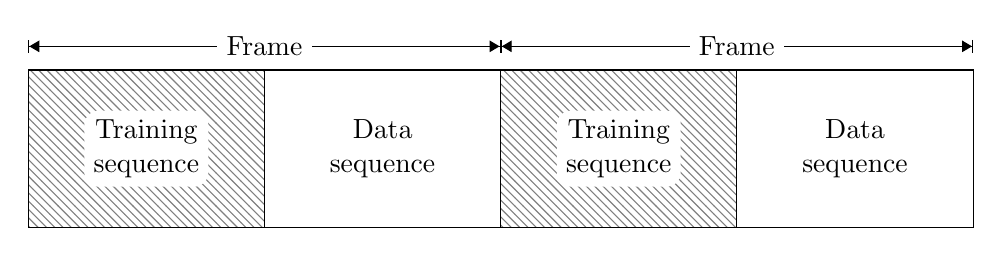
\begin{tikzpicture}
		\foreach \x [count=\n] in {0,6}{
			\begin{scope}[xshift=\x cm]
				\draw[pattern=north west lines, pattern color=gray] (0,0) rectangle node[fill=white, rounded corners=0.5em, align=center]{Training\\sequence} ++(3,2);
				\draw (3,0) rectangle node[align=center]{Data\\sequence} ++(3,2);
				\draw[{Bar}{Triangle}-{Triangle}{Bar}] (0,2.3) -- ++(6,0) node[midway, fill=white]{Frame};
			\end{scope}
		}
	\end{tikzpicture}
\end{document}
